

\documentclass[journal]{IEEEtran}

\usepackage{aligned-overset}












\ifCLASSINFOpdf
 
\else

\fi





%

\hyphenation{op-tical net-works semi-conduc-tor}


\begin{document}



\title{Report for Reading Project\\ A Generalized Path Integral Control Approach to Reinforcement Learning}





\author{Yunian Pan}




% make the title area
\maketitle

% As a general rule, do not put math, special symbols or citations
% in the abstract or keywords.
\begin{abstract}

This Report presents the substances of the paper "A Generalized Path Integral Control Approach to Reinforcement Learning", reinforcement learning has recently moved towards
combining classical techniques from optimal control and dynamic programming with modern learning techniques from statistical estimation theory in order to develop more scalable algorithms
with higher efficiency and fewer open parameters, the paper suggests to use the framework of stochastic optimal control with path integrals calle $PI^2$ to do parameterized policy approximation,  
 value function estimation and optimal control based on the stochastic Hamilton-Jacobi-Bellman (HJB) equations.
 
The algorithm's only parameter is the exploration noise, it can be conceived of as model-based, hybrid, or even model free,
depending on how the learning task is structured. 
The update equations have no danger of
numerical instabilities because neither matrix inversions nor gradient learning rates are required. 

The algorithm demonstrates interesting similarities with previous RL research in the framework
of probability matching and provides intuition why the slightly heuristically motivated probability
matching approach can actually perform well. 
There are some empirical evaluations demonstrate significant performance improvements over gradient-based policy learning and scalability to high-dimensional
control problems, and a simulation was presented in the end.

In general,
Policy Improvement with Path Integrals ($\mbox{PI}^2$) offers currently one of the most efficient, numerically robust, and easy to implement algorithms for RL based on trajectory roll-outs.
\end{abstract}
\ \\
% Note that keywords are not normally used for peerreview papers.
\begin{IEEEkeywords}
stochastic optimal control, reinforcement learning, parameterized policies, path integrals.
\end{IEEEkeywords}






% For peer review papers, you can put extra information on the cover
% page as needed:
% \ifCLASSOPTIONpeerreview
% \begin{center} \bfseries EDICS Category: 3-BBND \end{center}
% \fi
%
% For peerreview papers, this IEEEtran command inserts a page break and
% creates the second title. It will be ignored for other modes.
\IEEEpeerreviewmaketitle


\ \\
\section{Introduction}

\ \\

\IEEEPARstart{R}{einforcement} learning (RL) is under the danger of the curse of dimensionality in many cases such as humanoid robotic system. There are classical Value Iteration methods which offer possible
approach by function approximation, yet it remains problematic under non-stationary iterative learning when the dimension is too high. 

Alternatively, there are researchers developing different methods to improve this framework. 
Such as direct policy learning from trajectory roll-outs, which has made significantl progress but can still become numerically brittle and full of open tuning parameters in complex learning problems. 
In new developments, RL researchers have started to combine the well-developed methods from statistical learning and empirical inference with classical RL approaches in order to minimize tuning parameters and numerical problems, 
such that ultimately more efficient algorithms can be developed that scale to significantly more complex learning
system, there were a bunch of researchers working on it.

Spirited by the latter ideas, a new algorithm called Policy Improvement with Path Integrals (PI$^2$), derived from the stochastic optimal control and path integrals based on the original work of Kappen(2007) and Broek et al.(2008) 
was addressed in the paper. The algorithm makes connections between value function approximation through HJB and direct policy learning through approximating a path integral, thus it solves statistical inference
problems from sample roll-outs. 

It's simple formed, numerically robust in high dimensional problems, with no open algorithmic tuning parameters except exploration noise. What's more, it makes interesting connection to previous work on RL based on
probability matching and motivates why probability matching algorithms can be successful.






\ \\
\section{Theoretical development}
\ \\
The goal in stochastic optimal control framework is to control a stochastic dynamical system while
minimizing a performance criterion. Stochastic dynamical system means there are uncertain noise affecting the transition of states at each time step, 
while performance criterion is the characteristic to be measured of how well the solution to corresponding problems performs.
Stochastic optimal control can be thought as a constrained optimization problem in which the constrains corresponds to stochastic dynamical systems.
Following the structure of the paper, this part mainly addresses the derivation of stochastic optimal control with path integral.
\ \\

\subsection{Stochastic Optimal Control Definition and Notation}
\ \\
Since most of the theoretic notations in this paper are from trajectory-based optimal control, in order to creat as much overlaps as possible with
standard RL notations as Sutton proposed, a finite horizon cost function for a trajectory $\tau_i$(which can also be a piece of a trajectory) 
starting at time $t_i$ in state $x_{t_i}$ and ending at time $t_N$ is defined as follows, the subscripts for $t$ is for convenience of discretization:

\begin{equation}
  R(\tau_i)=\Phi_{t_N} + \int_{t_i}^{t_N}r_t dt
  \label{cost}
\end{equation}

where $\Phi_{t_N} = \Phi(x_{t_N})$ denotes the terminal reward at time $t_N$ and $r_t$ denotes the immediate cost at time t. In stochastic optimal control
as Stengel proposed in 1994, the goal is to find a control $u_t$ that minimizing the value function:

\begin{equation}
  V(x_{t_i})=V_{t_i} = \min_{u_{t_i:t_N}} E_{\tau_i} [R(\tau_i)]
  \label{valuefunc}
\end{equation}

Since the expectation $E_{\tau_i}$ is taken over all trajectories starting at $x_{t_i}$, we naturally think about a integral over all probability of trajectories,
which will be mentioned later.
First let's consider a general class of control systems, in other words, a general constraint:

\begin{equation}
  \dot{x}_t = f(x_t,t)+G(x_t)(u_t +\epsilon_t) = f_t +G_t (u_t +\epsilon_t)
  \label{dynamicfunc}
\end{equation}

with $x_t \in R^{n×\times 1}$ denoting the state of the system, $G_t = G(x_t ) \in R^{n\times p}$ the control matrix, $f_t = f(x_t ) \in R^{n×\times 1} $ the passive dynamics, $u_t \in R^{p×\times 1}$ the control vector and $\epsilon_t \in R^{p×\times1}$ Gaussian noise with variance $\Sigma_{\epsilon}$. As immediate cost we consider:

\begin{equation}
  r_t = r(x_t,u_t,t) = q_t + \frac{1}{2} u_t^{\top} R u_t
  \label{immediate cost}
\end{equation}

where $q_t = q(x_t,t)$ is an arbitrary state-dependent cost function, and R is the positive semi-definite weight matrix of the quadratic control cost. 
The stochastic HJB equation (Stengel, 1994; Fleming and Soner, 2006) associated with this stochastic optimal control problem is expressed as follows:

\begin{equation}
  -\partial_t V_t = \min_u (r_t + (\nabla_xV_t)^{\top}F_t + \frac{1}{2}trace((\nabla_{xx}V_t)G_t\Sigma_{\epsilon}G_t^{\top}))
  \label{HJB}
\end{equation}

This is done by second order Taylor approximation, where we assume that the noise is Gaussian White noise. To specify in this case, the derivation
is as follows:

By Bellman's principle of optimality, within a very little time interval $dt$, we have

\begin{equation}
  \begin{aligned}
  V_t  = \min E [{V_{t+dt} + \int_{t}^{t+dt} r_t dt}]   \\
  V_t dt  = \min E [\int_{t}^{t+dt} r_t dt+ V_t dt + (\nabla_x V_t)\dot{x} dt  \\ + \partial_tV_t + \dot{x}^{\top}(\nabla_{xx} V_t)\dot{x} dt^2] \nonumber \\
  -\partial_tV_t  = \min E [r_t + (\nabla_x V_t)\dot{x} + \dot{x}^{\top}(\nabla_{xx} V_t)\dot{x} dt]
  \end{aligned}
\end{equation}

* Comment here, suppose we already did the time discretization such that we can leverage Bellman's principle, actually we can drop out integration of $r_t dt$, instead write $r_t \Delta t$ 

Define $f(x_t,t)+G(x_t)u_t$ as $F_t$, $\epsilon_t\epsilon_t^{\top}$ as $\Sigma_{\epsilon}$, leveraging some nice properties of Gaussian white noise, we can cancel the $dt$ term and turned this equation into the 
HJB form:

\begin{equation}
  \begin{aligned}
    -\partial_tV_t  = \min E [r_t + (\nabla_x V_t)F_t +  (\nabla_x V_t)G_t \epsilon_t \\
    + (F_t+G_t \epsilon_t))^{\top}(\nabla_{xx} V_t)(F_t+G_t \epsilon_t)) dt] \nonumber \\
    \quad \\
    -\partial_tV_t = \min \{ E [r_t + (\nabla_x V_t)F_t + (G_t \epsilon_t)^{\top}(\nabla_{xx} V_t)(G_t \epsilon_t)dt] \\
 + E[(\nabla_x V_t)G_t \epsilon_t + F_t^{\top}(\nabla_{xx} V_t)F_tdt + 2G_t \epsilon_t^{\top}(\nabla_{xx} V_t)F_tdt ] \} \\
 \quad 
  \end{aligned}
\end{equation}

while under certain control, $r_t + (\nabla_x V_t)F_t$ is certain and can be taken out side of the expectation. Introducing trace operation so that we can switch the order of matrices multiplication, 
and according to $\int E(\epsilon_t\epsilon_t^{\top} dt ) = \Sigma_{\epsilon}$, the 3rd term can be also taken out of the expectation. The other terms all go to 0 as either dt is very small or 
Gaussian noise is zero mean value.

We inset immediate cost $\ref{immediate cost}$ into HJB equation $\ref{HJB}$, the gradient of the expression inside the parenthesis is taken with respect to controls u and set to zero, thus resulting the optimal control
by the equation:

\begin{equation}
  u(x_t)=u_t =-R^{-1}G_t^{\top}(\nabla_{x_t}V_t)
  \label{optimal control}
\end{equation}

insert $\ref{optimal control}$ into HJB $\ref{HJB}$ to substitute the 2nd term, we get a nonlinear and second order Partial Differential Equation(PDE) as follows:

\begin{equation}
  \begin{aligned}
  -\partial_t V_t = q_t + (\nabla_xV_t)^{\top}f_t -\frac{1}{2}(\nabla_xV_t)^{\top}G_tRd^{-1}G_t^{\top}(\nabla_{x_t}V_t) \\
   + \frac{1}{2}trace((\nabla_{xx}V_t)G_t\Sigma_{\epsilon}G_t^{\top})
  \label{nonlinear PDE}
  \end{aligned}
\end{equation}

The $\nabla_x$ and $\nabla_{xx}$ symbols refer to the Jacobian and Hessian, respectively, of the value function with respect to the state x, while ∂t is the partial derivative with respect to time. For notational compactness, 
we will mostly use subscripted symbols to denote time and state dependencies, as introduced in the equations above.

Thus we have formulated this general case of stochastic optimal control into a PDE problem, which is nonlinear and hard to solve, next step is to change the variable and formulate another
linear PDE.
 \ \\

\subsection{Transformation of HJB into a Linear PDE}
\ \\

In order to find a solution to the PDE above, we use an exponential transformation of the value function:

\begin{equation}
  V_t = -\lambda \log \Psi_t \nonumber
\end{equation}

Given the logarithmic transformation, the partial deravatives can be written as follows:

\begin{equation}
  \partial_tV_t = -\lambda \frac{1}{\Psi_t}\partial_t \Psi_t \nonumber
\end{equation}

\begin{equation}
  \nabla_xV_t = -\lambda \frac{1}{\Psi_t}\nabla_x \Psi_t \nonumber
\end{equation}

\begin{equation}
  \nabla_{xx}V_t = \lambda \frac{1}{\Psi_t^2}\nabla_x \Psi_t\nabla_x \Psi_t^{\top} -\lambda \frac{1}{\Psi_t}\nabla_{xx} \Psi_t \nonumber
\end{equation}

Inseting the equations above into nonlinear PDE $\ref{nonlinear PDE}$, we are replacing $\partial_tV_t$, $\nabla_xV_t$ and $\nabla_{xx}V_t$,
we obtain:

\begin{equation}
  \begin{aligned}
  \lambda \frac{1}{\Psi_t}\partial_t \Psi_t = \min_u (r_t -\lambda \frac{1}{\Psi_t}(\nabla_x \Psi_t )^{\top}f_t \\ -\frac{\lambda^2}{2\Psi^2}(\nabla_x \Psi_t )^{\top}G_tR^{-1}G_t^{\top}(\nabla_{x_t}V_t) \\
   + \frac{1}{2}trace(\Gamma) 
  \label{nonlinear PDE2}
  \end{aligned}
\end{equation}

Where $\Gamma$ is expressed as:

\begin{equation}
  \Gamma = (\lambda\frac{1}{\Psi_t^2}\nabla_x \Psi_t\nabla_x \Psi_t^{\top} - \lambda \frac{1}{\Psi_t} \nabla_{xx}\Psi_t)G_t\Sigma_{\epsilon} G_t^{\top} \nonumber
\end{equation}

the trace of $\Gamma $ is therefore:

\begin{equation}
  \begin{aligned}
  trace(\Gamma) = \lambda \frac{1}{\Psi^2}trace(\nabla_x\Psi_t^{\top} G_t \Sigma_{\epsilon} G_t \nabla_x\Psi_t) \\ - \lambda \frac{1}{\Psi}trace(\nabla_{xx}\Psi_t)G_t\Sigma_{\epsilon} G_t^{\top})
   \label{gamma1}  
\end{aligned}
\end{equation}

Here in the paper there's a great observation made by the authors, that the first term of $\ref{gamma1}$ and the second term of $\ref{nonlinear PDE2}$ can be canceled out,
if we assume $\lambda R^{-1} = \Sigma_{\epsilon}$, which implies the simplification:

\begin{equation}
  \lambda G_t R^{-1}G_t^{\top} = G_t \Sigma_{\epsilon}G_t^{\top} = \Sigma(x_t)
  \label{assumption1}
\end{equation}

the intuition behind this assumption is introduced by Kappen, 2007 and also Broek et al., 2008. $\lambda $ is an arbitary positive value, since the weight control matrix R is inverse proportional to the variance of the noise, 
a high variance control input implies cheap control cost, while small variance control inputs have high control cost, this relationship is logical correct from a control theoretic stand point,
High variance means the control is under a large disturbance and it takes a large value of u to bring the system back to a desirable state, thus resulting low control cost in R.

This assumption makes sense to some degree, yet we are not sure what nature will reveal, the reliability of this inverse proportional relationship is only worth discussion or comparison while they can
result in reliable algorithms, this assumption significantly reduces the comlexity of the PDE and theoretically makes sense, and it's generalizable. 

So far with the simplification, $\ref{nonlinear PDE2}$ can be reduced to:

\begin{equation}
  -\partial_t \Psi_t = - \frac{1}{\lambda } q_t \Psi_t + f_t^{\top}(\nabla_x \Psi_t) + \frac{1}{2} trace((\nabla_{xx}\Psi_t)G_t \Sigma G_t^{\top})
  \label{reduced form1}
\end{equation}

with boundary condition $\Psi_{t_N} = \exp(-\frac{1}{\lambda} \phi_{t_N})$, as the terminal cost is fixed. The PDE in $\ref{reduced form1}$ 
corresponds to the so called Chapman Kolmogorov PDE.solutions of (9) cannot be found in general for general nonlinear systems and cost functions. How- ever, 
there is a connection between solutions of PDEs and their representation as stochastic differential equation (SDEs), that is mathematically expressed by the 
Feynman-Kac formula (Øksendal, 2003; Yong, 1997). 
The Feynman-Kac formula can be used to 
find distributions of random processes which solve certain SDEs as well as to propose numerical methods for solving certain PDEs. Applying the Feynman-Kac theorem, 
the solution of (9) is:

\begin{equation}
\Psi_{t_i} = E_{\tau_i}(\Psi_{t_N}e^{-\int_{t_i}^{t_N}\frac{1}{\lambda}q_tdt}) = E_{\tau_i}[\exp(-\frac{1}{\lambda}\phi_{t_N}-\frac{1}{\lambda}\int_{t_i}^{t_N}q_tdt)]
\end{equation}

Thus, we have transformed our stochastic optimal control problem into the approximation problem of a path integral. 
With a view towards a discrete time approximation, which will be needed for numerical implementations, the solution above can be formulated as:

\begin{equation}
  \Psi_{t_i} = \lim_{dt\to 0}\int p(\tau_i|x_{t_i}) \exp[-\frac{1}{\lambda}(\phi_{t_N}+\sum_{j=i}^{N-1}q_{t_j}dt)]d\tau_i
  \label{solution1}
\end{equation}

where $\tau_i = (x_{t_i} , ....., x_{t_N} )$ is a sample path (or trajectory piece) starting at state $x_{t_i}$
$p(\tau_i|x_i)$ is the probability of sample path τi conditioned on the start state $x_{t_i}$. 
Since Equation $\ref{solution1}$ provides the exponential cost to go $\Psi_{t_i}$ in state xti , the integration above is taken with respect to sample paths $\tau_i = (x_{t_i} , ....., x_{t_N} )$. 
The differential termd $\tau_i$ is defined as $d\tau_i =(dx_{t_i},.....,dx_{t_N})$. Evaluation of the stochastic integral in $\ref{solution1}$ requires the specification of $p(\tau_i|x_i)$, 
in other words without generalization given a dynamics we have to evaluate the trajectories step by step, which demandes enormous conputation. 
How to simplify this process is crucial, which is the topic of our analysis in the next part.


\ \\
\subsection{Generalized Path Integral Formulation}
  \ \\

To develop our algorithms, we will need to consider a more general development of the path integral approach to stochastic optimal control than presented in Kappen (2007) and Broek et al. (2008). 
In particular, we have to address that in many stochastic dynamical systems,
 the control transition matrix $G_t$ is state dependent and its structure depends on the partition of the state in directly and non-directly actuated parts. Since only some of the states are directly controlled, the state vector
 is partitioned into $x = [x(m)^T \ x(c)^T ]^T$ with $x(m) \in R^{k\times 1}$ the non-directly actuated part and $x(c) \in R^{l\times 1}$ the directly actuated part. Subsequently, the passive dynamics term and the control transition
 matrix can be partitioned as $f_t =[f_t^{(m)} f_t^{(c)} ]^{\top}$ with $f_m \in R^{k\times 1}$, $f_c \in R^{l\times 1}$ and $G_t = [0_{k\times p} \ {G_t^{(c)}}^{\top}]$, with $G^{(c)} \in R^{l\times p}$. The discretized state space representation of such systems is given as:
 
 \begin{equation}
  x_{t_{i+1}} =x_{t_i} +f_{t_i}dt+G_{t_i} (u_{t_i}dt+\sqrt{dt}\epsilon_{t_i})\nonumber
 \end{equation}

 * According to Eular's scheme for diffusions, when we are simulating a SDE, there exists a $\sqrt{dt}$ because the discretization step is derived from the second order Taylor approximation around the point $x_{t_i}$ to the point $x_{t_{i+1}}$ with respect to both time and stochastic term, stopping at the second order,
 and ignore some terms that go to 0, see Ito's lemma.
 
 In partitioned vector form, the equation can be written as:

 \begin{equation}
 \begin{pmatrix}x_{t_{i+1}}^{(m)} \\ x_{t_{i+1}}^{(c)} \end{pmatrix}=\begin{pmatrix}x_{t_{i}}^{(m)} \\ x_{t_{i}}^{(c)} \end{pmatrix} +\begin{pmatrix}f_{t_i}^{(m)} \\ f_{t_i}^{(c)}\end{pmatrix}dt+\begin{pmatrix}0_{k\times p}\\G_{t_i}^{(c)}  \end{pmatrix} (u_{t_i}dt+\sqrt{dt}\epsilon_{t_i})
 \label{discretized form}
\end{equation}

Essentially the stochastic dynamics are partitioned into controlled equations in which the state $x_{t_{i+1}}^{(c)}$
is directly actuated and the uncontrolled equations in which the state $x_{t_{i+1}}^{(m)}$ is not directly actuated. 
Since stochasticity is only added in the directly actuated terms (c) of $\ref{discretized form}$, we can develop $p(\tau_i|x_i)$ as follows.

\begin{equation}
  \begin{aligned}
    p(\tau_i|x_i) & =  p(\tau_{i+1}|x_{t_i})  \\ 
    & = p(x_{t_{i+1}},\ldots, x_{t_N}|x_{t_i}) \\
    & = \prod_{j = i}^{N-1} p (x_{t_{j+1}}|x_{t_i}) \nonumber
  \end{aligned}
\end{equation}


where we exploited the fact that the start state $x_{t_i}$ of a trajectory is given and does not contribute to its probability. 
For systems where the control has lower dimensionality than the state $\ref{discretized form}$, the transition probabilities $p (x_{t_j+1} |x_{t_j} )$ are factorized as follows:

\begin{equation}
  \begin{aligned}
    p (x_{t_j+1} |x_{t_j} ) & =  p (x_{t_j+1}^{(c)} |x_{t_j} ) \cdot p (x_{t_j+1}^{(m)} |x_{t_j} ) \\ 
    & = p (x_{t_j+1}^{(c)} |x_{t_j}^{(c)}, x_{t_j}^{(m)} )\cdot p (x_{t_j+1}^{(m)} |x_{t_j}^{(c)}, x_{t_j}^{(m)}) \\
    & \propto p (x_{t_{j+1}}^{(c)}|x_{t_i}) 
  \end{aligned}
  \label{factorized transition probabilities}
\end{equation}


where we have used the fact that $p (x_{t_j+1}^{(m)} |x_{t_j}^{(c)}, x_{t_j}^{(m)})$ is the Dirac delta function, since $x_{t_j}^{(m)}$ can be 
computed deterministically from $x_{t_j}^{(c)}, x_{t_j}^{(m)}$. For all practical purposes, the transition probability of
the stochastic dynamics is reduced to the transition probability of the directly actuated part of the
state:

\begin{equation}
  \begin{aligned}
    p(\tau_i|x_i) & =  \prod_{j = i}^{N-1} p (x_{t_{j+1}}|x_{t_i})\\ 
    & \propto \prod_{j = i}^{N-1} p (x_{t_{j+1}}^{(c)}|x_{t_i})
  \end{aligned}
  \label{transition dynamic}
\end{equation}

Since we assume that the noise $\epsilon$ is zero mean Gaussian white noise distributed with variance $\Sigma_{\epsilon}$, where $\Sigma_{\epsilon} \in R^{l\times l}$,
the transition probability of the directly actuated part of the state is defined as:

\begin{equation}
  \begin{aligned}
    p (x_{t_j+1}^{(c)} |x_{t_j} ) =  \frac{1}{((2\pi)^{l} \cdot |\Sigma_{t_j}|)^{\frac{1}{2}}} \exp( -|| x_{t_j+1}^{(c)} - x_{t_j}^{(c)} - f_{t_j}^{(c)}dt||^2_{\Sigma_{t_j}})
  \end{aligned}
  \label{transition directly}
\end{equation}

where the covariance $\Sigma_{t_j} \in R^{l\times l}$ is expressed as $\Sigma_{t_j} = G_{t_j}^{(c)} \Sigma_{\epsilon}{G_{t_j}^{(c)}}^{\top} dt$. So we get trajectories' probabilities
as follows: 

\begin{equation}
  \begin{aligned}
    p(\tau_i|x_i) \propto \prod_{j = i}^{N-1}  \frac{1}{((2\pi)^{l} \cdot |\Sigma_{t_j}|)^{\frac{1}{2}}} \exp( -|| x_{t_j+1}^{(c)} - x_{t_j}^{(c)} - f_{t_j}^{(c)}dt||^2_{\Sigma_{t_j}})
  \end{aligned}
  \label{transition directly}
\end{equation}


incorporate the assumption $\ref{assumption1}$ about the relation between the control cost and the variance of the noise,  which needs to be adjusted to the controlled space as
$\Sigma_{t_j} = G_{t_j}^{(c)}\Sigma_{\epsilon}{G_{t_j}^{(c)}}^{\top}dt  = \lambda G_{t_j}^{(c)} R^{-1}{G_{t_j}^{(c)}}^{\top} dt = \lambda H_{t_j} dt $, thus obtain:

\begin{equation}
  \begin{aligned}
    p(\tau_i|x_i) \propto  \frac{1}{\prod_{j = i}^{N-1} ((2\pi)^{l} \cdot |\Sigma_{t_j}|)^{\frac{1}{2}}} \\ \exp( -\frac{1}{2\lambda}\sum_{j=i}^{N-1}|| \frac{x_{t_j+1}^{(c)} - x_{t_j}^{(c)}}{dt} - f_{t_j}^{(c)}||^2_{H_{t_j}}dt)
  \end{aligned}
  \label{transition directly}
\end{equation}


With this formulation of the probability of a trajectory, we can rewrite the the path integral $\ref{solution1}$ as:

\begin{equation}
  \begin{aligned}
  &\Psi_{t_i}  = \lim_{dt\to 0}\int \\ 
  &\frac{\exp[-\frac{1}{\lambda}(\phi_{t_N}+\sum_{j=i}^{N-1}q_{t_j}dt + \frac{1}{2}\sum_{j=i}^{N-1}|| \frac{x_{t_j+1}^{(c)} - x_{t_j}^{(c)}}{dt} - f_{t_j}^{(c)}||^2_{H_{t_j}})]}{\prod_{j = i}^{N-1} ((2\pi)^{l} \cdot |\Sigma_{t_j}|)^{\frac{1}{2}}}d\tau_i \nonumber \\
  &\Psi_{t_i}   = \lim_{dt\to 0}\int \frac{1}{D(\tau_i)}\exp(-\frac{1}{\lambda}S(\tau_i))d\tau_i^{(c)}
  \label{solution2}
  \end{aligned}
\end{equation}

where, we defined:

\begin{equation}
  S(\tau_i) = \phi_{t_N}+\sum_{j=i}^{N-1}q_{t_j}dt + \frac{1}{2}\sum_{j=i}^{N-1}|| \frac{x_{t_j+1}^{(c)} - x_{t_j}^{(c)}}{dt} - f_{t_j}^{(c)}||^2_{H_{t_j}} dt \nonumber 
\end{equation}

and

\begin{equation}
  D(\tau_i) = \prod_{j = i}^{N-1} ((2\pi)^{l} \cdot |\Sigma_{t_j}|)^{\frac{1}{2}}) \nonumber
\end{equation}

Note that the integration is over $d\tau_i^{(c)} = (dx_{t_i}^{(c)},\ldots,dx_{t_N}^{(c)})$, as the non-directly actuated states
can be integrated out due to the fact that the state transition of the non-directly actuated states is deterministic, 
and just added Dirac delta functions in the integral $\ref{factorized transition probabilities}$. 
Equation $\ref{solution2}$ is written in a more compact form as:

\begin{equation}
  \begin{aligned}
   \Psi_{t_i} & = \lim_{dt\to 0}\int \exp(-\frac{1}{\lambda}S(\tau_i) -\log D(\tau_i)) d\tau_i^{(c)} \\
 & = \lim_{dt\to 0}\int \exp(-\frac{1}{\lambda}Z(\tau_i)) d\tau_i^{(c)}  
  \label{solution3}
  \end{aligned}
\end{equation}

where $Z(\tau_i) = S(\tau_i)+\lambda \log D(\tau_i)$. It can be shown that this term is factorized in path dependent and path independent terms of the form:

\begin{equation}
  \begin{aligned}
   Z(\tau_i) = \tilde{S(\tau_i)}+ \frac{\lambda (N-i)l}{2} \log (2\pi dt \lambda)
  \end{aligned}
\end{equation}

Where $\tilde{S(\tau_i)} = S(\tau_i) + \frac{\lambda}{2} \sum_{j = i}^{N-1} \log H_{t_j}$. This formula is a required step for the derivation of next part,
the second term $\frac{\lambda (N-i)l}{2} \log (2\pi dt \lambda)$ can be a source of numerical instabilities especially in cases where fine discretization dt of 
stochastic dynamics is required. Yet it can be dropped out of the equation as will be mentioned later in section D. (Because it's states independent)


\subsection{Optimal Controls}

For every moment of time, the optimal controls are given as $u_{t_i} = -R^{-1} G_{t_i}^{\top} (\nabla_{x_{t_i}}V_{t_i})$, Due to the
exponential transformation of the value function, the equation of the optimal controls can be written 


\begin{equation}
  \begin{aligned}
   u_{t_i} = \lambda R^{-1} G_{t_i} \frac{\nabla_{x_{t_i}}\Psi_{t_i}}{\Psi_{t_i}}  \nonumber
  \end{aligned}
\end{equation}


After substituting $\Psi_{t_i}$ with $\ref{solution3}$ and canceling the state independent terms of the cost we have:


\begin{equation}
  \begin{aligned}
   u_{t_i} = \lim_{dt \to 0 } (\lambda R^{-1} G_{t_i} \frac{\nabla_{x_{t_i}}\int \exp(-\frac{1}{\lambda}\tilde{S}(\tau_i)) d\tau_i^{(c)} }{\int \exp(-\frac{1}{\lambda}\tilde{S}(\tau_i)) d\tau_i^{(c)} } ) \nonumber
  \end{aligned}
\end{equation}

With further analysis, we will obtain another simplified version of the equation above, The proof of lemma 1 of appendix A precisely shows how the trajectory independent term
$\frac{\lambda (N-i)l}{2} \log (2\pi dt \lambda)$ was taken out of the and gradient and then taken out of the integration and canceled out.


\begin{equation}
  \begin{aligned}
   u_{t_i} = \int P(\tau_i) u_L(\tau_i) d\tau_i^{(c)}  
  \end{aligned}
\end{equation}

with the probability $P(\tau_i)$ defined as:

\begin{equation}
  \begin{aligned}
   P(\tau_i) = \frac{e^{-\frac{1}{\lambda}\tilde{S}(\tau_i)}  }{\int e^{-\frac{1}{\lambda}\tilde{S}(\tau_i)}d\tau_i}
  \end{aligned}
\end{equation}

\begin{equation}
  \begin{aligned}
    u_L(\tau_i) = -R^{-1} {G_{t_i}^{(c)}}^{\top} \lim_{dt\to 0 }(\nabla_{x_{t_i}^{(c)}}\tilde{S}(\tau_i))
  \end{aligned}
\end{equation}

The definitions above are not groundless as they are obtained from what the proof of lemma 1 finally leads to, also they are intuitively understandable
as $\tilde{S}(\tau_i)$ represents all the trajectory dependent parts of the value function and $u_L(\tau_i)$ has a very similiar form with the optimal control derived in
in section A.

The path cost $\tilde{S}(\tau_i)$ is a generalized version which only considered systems with state independent control transition $G_{t_i}$. To 
find the local controls $u_L(\tau_i)$ we have to calculate the $\lim_{dt\to 0 }(\nabla_{x_{t_i}^{(c)}}\tilde{S}(\tau_i))$

The proof of lemma 2 of appendix A precisely gives the analytical steps of how we get the term $\nabla_{x_{t_i}^{(c)}}\tilde{S}(\tau_i)$ solved in following form:

\begin{equation}
  \begin{aligned}
    \nabla_{x_{t_i}^{(c)}}\tilde{S}(\tau_i) = - H_{t_i}^{-1} (G_{t_i}^{(c)}\epsilon_{t_i} - b_{t_i})
  \end{aligned}
\end{equation}

Where the function $b(x_{t_i})$ defined as $\lambda H(x_{t_i})\Phi_{t_i}$ with $H_{t_i} = G_{t_i}^{(c)} R^{-1} {G_{t_i}^{(c)}}^{\top}$ and the quantity $\Phi_{t_i} \in R^{l \times 1}$
is expressed as:

\begin{equation}
  \begin{aligned}
  \Phi_{t_i} = \frac{1}{2} \begin{bmatrix} trace(H_{t_i}^{-1} \partial_{x_{t_i}^{c1}} H_{t_i}) \\trace(H_{t_i}^{-1} \partial_{x_{t_i}^{c2}} H_{t_i}) \\\vdots \\ trace(H_{t_i}^{-1} \partial_{x_{t_i}^{cl}} H_{t_i})\end{bmatrix} \nonumber 
  \end{aligned}
\end{equation}

The proof is a long story with pure mathematical work, briefly we calculate the jacobians of 4 terms respectively, several identities are used such as $\partial \det(A) = \det(A) Tr(A^{-1}\partial A )$. 

The local control can now be expressed as:

\begin{equation}
  u_L(\tau_i) = R^{-1} {G_{t_i}^{(c)}}^{\top} H_{t_i}^{-1}(G_{t_i}^{(c)}\epsilon_{t_i} - b_{t_i})
\end{equation}


substituting $H_{t_i}^{-1}$ with $({G_{t_i}^{(c)}} R^{-1} {G_{t_i}^{(c)}}^{\top})^{-1}$, we get our main result for the local 
controls of the sampled path for the generalized path integral formulation:

\begin{equation}
  u_L(\tau_i) = R^{-1} {G_{t_i}^{(c)}}^{\top} ({G_{t_i}^{(c)}} R^{-1} {G_{t_i}^{(c)}}^{\top})^{-1}(G_{t_i}^{(c)}\epsilon_{t_i} - b_{t_i})
\end{equation}



The equations above form the solution for the generalized path integral stochastic optimal control problem.
 Given that this result is of general value and constitutes the foundation to derive our reinforcement learning algorithm in the next section,
 but also many other special cases can be derived from it.

 So what comes first is a model-based approach, which demands for model of the system dynamics, the cost function, knowledge of the system’s noise process, 
 and a mechanism to generate trajectories $\tau_i$, the computations of the optimal controls requires knowledge of $\epsilon$, which can be obtained in 2 ways.
 with trajectories sampled from a random number generator or generated by a real system, the noise can be computed from the difference between the actual and the 
 predicted system behavior, i.e. $G_{t_i}^{(c)}\epsilon_i = \dot{x}   - \hat{\dot{x}}  = \dot{x_{t_i}}  - (f_{t_i} + G_{t_i} u_{t_i} ).$, where computing the $\hat{\dot{x}}$
 requires the knowledge of the system dynamics behavior.






\subsection{Special Cases}

First let's see some cases of special formed dynamical systems applying the path integral approach, preparing for the reinforcement learning algorithm.

 \ \\
\subsubsection{systems with one dimensional directly actuated states}
\ \\

The generalized formulation of stochastic optimal control with path integrals in Table 1 can be
applied to a variety of stochastic dynamical systems with different types of control transition matrices

\begin{table}
 \caption{}
 \label{table 1}
  \begin{itemize}
    \item[$\bullet$] Given: 
    \begin{itemize}
      
      \item the system dynamics: $\dot{x}_t = f(x_t,t)+G(x_t)(u_t +\epsilon_t) = f_t +G_t (u_t +\epsilon_t)$
      \ \\
      \item The immediate cost: $r_t = r(x_t,u_t,t) = q_t + \frac{1}{2} u_t^{\top} R u_t$
      \ \\
      \item A terminal cost term $\Phi_{t_N}$
      \ \\
      \item The variance $\Sigma_{\epsilon}$ of the mean-zero noise $\epsilon_t$
      \ \\
      \item Trajectory starting at $t_i$ and ending at $t_N$ : $\tau_i =(x_{t_i}, \ldots ,x_{t_N})$
      \ \\
      \item A partitioning of the system dynamics into (c) controlled and (m) uncontrolled equations, where n = c + m is the dimensionality of the state $x_t$ 
    \end{itemize}  
     \ \\
    \item[$\bullet$] Optimal Controls:
    \begin{itemize}
      
      \item optimal controls at every time step $t_i$: $u_{t_i} = \int P(\tau_i) u_L(\tau_i) d\tau_i^{(c)}  $
      \ \\
      \item Probability of a trajectory: $P(\tau_i) = \frac{e^{-\frac{1}{\lambda}\tilde{S}(\tau_i)}  }{\int e^{-\frac{1}{\lambda}\tilde{S}(\tau_i)}d\tau_i}$ 
      \ \\
      \item Generalized trajectory cost: $\tilde{S}(\tau_i) = S(\tau_i) + \frac{\lambda}{2} \sum_{j = i}^{N-1} \log |H_{t_j}|$
       \ \\
      \item Local controls: $u_L(\tau_i) = R^{-1} {G_{t_i}^{(c)}}^{\top} ({G_{t_i}^{(c)}} R^{-1} {G_{t_i}^{(c)}}^{\top})^{-1}(G_{t_i}^{(c)}\epsilon_{t_i} - b_{t_i})$
    \end{itemize} 
  \end{itemize}

\end{table}

control transition matrix $G_t$ with 1 dimensional actuated system becomes a row vector. 

The optimal control is:

\begin{equation}
  u_L(\tau_i) = \frac{R^{-1}{g_t^{(c)}}}{{g_t^{(c)}}^{\top}R^{-1}g_t^{(c)}} ({g_t^{(c)}}^{\top}\epsilon_t - b_t)
\end{equation}

\ \\
\subsubsection{systems with one dimensional directly actuated states}
\ \\

The generalized formula of the local controls (20) was derived for the case where the control transition matrix is state dependent and its dimensionality is $G_{t_i}^{(c)} \in R^{l\times p}$  with l < n and p the dimensionality 
of the control. There are many special cases of stochastic dynamical systems in optimal control and robotic applications that belong into this general class. For systems having a state
dependent control transition matrix that is square the local controls can be significantly simplified to following form:

\begin{equation}
  u_L(\tau_i) = \epsilon_{t_i} - {G_{t_i}^{(c)}}^{-1} b_{t_i}
  \label{21}
\end{equation}

Interestingly a rather general class of mechanical systems such as rigid-body and multi-body dynamics fall into this category. When these mechanical systems are expressed in state space, the control transition matrix 
will be equal to rigid body inertia matrix.

Another special case is when $G_t$ is a constant and the local controls becomes:

\begin{equation}
  u_L(\tau_i) = R^{-1} {G^{(c)}}^{\top} ({G^{(c)}} R^{-1} {G^{(c)}}^{\top})^{-1}(G^{(c)}\epsilon_{t_i})
  \label{22}
\end{equation}

Or, even if $G_{t_i}^{(c)}$ is square and state independent, $G_{t_i}^{(c)} = G^{(c)} \in R^{l \times l}$, then we have:

\begin{equation}
  u_L(\tau_i) = \epsilon_{t_i} 
  \label{23}
\end{equation}

So that the local optimal control turn into noise at $t_i$.

Yet the algorithm in the paper allows a broader application in various areas where the control transtion matrix is typically partitioned into directly and non-directly actuated states,
and typically also state dependent.

\ \\
\subsubsection{systems with one dimensional directly actuated states}
\ \\
In this class of stochastic systems, the control transition matrix is not partitioned and, therefore, the
control u directly affects all the states. In this case $G_{t_i}$ is a square matrix and we obtain:

\begin{equation}
  u_L(\tau_i) = \epsilon_{t_i} - {G_{t_i}^{(c)}}^{-1} b_{t_i}
\end{equation}

With 

\begin{equation}
  b_{t_i} = \lambda H_{t_i} \Phi_{t_i} \nonumber 
 \end{equation}

and


\begin{equation}
 (\Phi_{t_i})_j =  \frac{1}{2} trace ({H_{t_i}}^{-1}({\partial_{x_{t_i}}}_j H_{t_i} ) )\nonumber 
\end{equation}
 
 For this fully actuated state space, there are subclasses of dynamical systems with square and/or state independent control transition matrix. The local controls for these cases are found by just
 (c) substituting $G_{t_i}$ with $G_{t_i}$ in $\ref{21}$, $\ref{22}$ and $\ref{23}$.
 
 So far so good, we are done with the stochastic optimal control part and get a bunch of results as tools, in the next section we are going to leverge these tools and results to develop the reinforcement 
 learning algorithm PI$^2$.


\ \\
\section{Reinforcement Learning with Parameterized Polices}
\ \\

Equipped with the theoretical framework of stochastic optimal control with path integrals, we can now turn to its application to reinforcement learning with parameterized policies. 
Since the beginning of actorcritic algorithms. one goal of reinforcement learning has been to learn compact policy representations, for example, with neural networks as in the early 
days of machine learning, or with general parameterizations. Parameterized policies have much fewer parameters than the classical time-indexed approach of optimal control, where every 
time step has its own set of parameters, i.e., the optimal controls at this time step. Usually, function approximation techniques are used to represent the optimal controls and the 
open parameters of the function approximator become the policy parameters. Function approximators use a state representation as input and not an explicit time dependent representation. 
This representation allows generalization across states and promises to achieve better generalization of the control policy to a larger state space, such that policies become reusable 
and do not have to be recomputed in every new situation.

As can be seen from the previous sections, the classical time-based optimal control strategy can also be developed since the results are time-indexed, which means they are time dependent.
However with a minor re-interpretation of the approach and some small mathematical adjustments, we can carry it over to parameterized policies and reinforcement learning.


\subsection{Parameterized Policies}

Focusing on direct policy learning, where the parameters of the policy are adjusted by a learning rule directly, and not indirectly as in value function approaches of classical reinforcement learning
developed by Sutton and Barto.

(*The pros and cons of direct vs. indirect policy learning has provoked many discussion, a general point is that indirect learning makes fuller use of the real world experience, which usually contributes to get better
policy with fewer environment interactions, while direct policy learning is simpler formed and its performance wouldn't be affected by bad models.)

Direct policy learning usually assumes a general cost function in the form of:

\begin{equation}
  J(x_0) = \int p(\tau_0)R(\tau_0)d\tau_0
\end{equation}

which is optimized over states-action trajectories $\tau_0 = (x_{t_0}, \alpha_{t_0}, \ldots, \alpha_{t_{N-1}} ,x_{t_N})$. Under the first order Markov
property, the probability of a trajectory is:

\begin{equation}
  p(\tau_i)=p(x_{t_i} )\prod_{j = i}^{N-1} p(x_{t_{j+1}} |x_{t_j} ,\alpha_{t_j} )p(\alpha_{t_j} |x_{t_j} )
\end{equation}

Both the state transition and the policy are assumed to be stochastic. The particular formulation of the stochastic policy is a design parameter, motivated by the application domain, 
analytical convenience, and the need to inject exploration during learning. For continuous state action domains, Gaussian distributions are most commonly chosen.

Usually for continuous state-action domains, the stochastic policies are parameterized as:

\begin{equation}
   \alpha_{t_i} = g_{t_i}^{\top} (\theta + \epsilon_{t_i})
\end{equation}

with $g_{t_i}$ denoting a vector of basis functions and $\theta$ the parameter vector. For Gaussian noise $\epsilon$ the probability of an action is normal distributed with mean value vector $\theta^{\top} g_{t_i}$ and variance matrix $\Sigma_{t_i} = g_{t_i}^{\top} \Sigma_{\epsilon} g_{t_i}$

\ \\
\subsection{From DMPs to PI$^2$}
\ \\
As we are interested in model-free learning, we should follow the structure that optimize control policies which represent desired trajectories. 
The special case  Dynamic Movement Primitives(DMPs) is used in this paper to illustrate , which are expressed as follows:

\begin{equation}
  \begin{aligned}
     \frac{1}{\tau} \dot{z_t} & = f_t + g_t^{\top}(\theta + \epsilon_t) \\
     \frac{1}{\tau} \dot{y_t} & = z_t \\
     \frac{1}{\tau} \dot{x_t} & = -\alpha x_t \\ 
     f_t & = \alpha_z(\beta_z(g-y_t)- z_t).  \nonumber
  \end{aligned}
  \label{DMPs}
\end{equation}

Essentially, these policies code a learnable point attractor for a movement from $y_{t_0}$ to goal $g$, where $\theta$ determines the shape of the attractor; 
$y_t$, $\dot{y_t}$ denote the position and velocity of the trajectory, while $z_t$ , $x_t$ are internal states. The basis function can be defined by a piecewise
linear function approximator with Gaussian weight kernels:

\begin{equation}
  \begin{aligned}
     |g_t|_j &= \frac{w_jx_t}{\sum_{k=1}^{p}w_k}(g-y_{t_0}) \\
     w_j & = \exp(0.5 h_j(x_t - c_j )^2) \nonumber 
  \end{aligned}
\end{equation}

Where $c_j$ is one of the Gaussian kernels. By varying $\theta$ the shape of the trajectory changes without changing the initial and final state.  

Start from this case, first by building blocks we can easily find out the directly actuated terms:

\begin{equation}
\begin{pmatrix} \dot{x_t} \\ \dot{y_t} \\ \dot{z_t} \end{pmatrix} = \begin{pmatrix} -\alpha x_t \\ z_t \\ \alpha_z(\beta_z(g-y_t)- z_t)+ g_t^{\top}(\theta + \epsilon_t) \end{pmatrix} + \begin{pmatrix} 0_{ 1 \times p} \\ 0_{ 1 \times p} \\ {g_{t_i}^{(c)}}^{\top}  \end{pmatrix}(\theta_t + \epsilon_t)
\end{equation}

The states are thus partitioned into the uncontrolled states and the controlled states. Here we write the path cost:


\begin{equation}
  \begin{aligned}
    \tilde{S(\tau_i)}& = \phi_{t_N}+\sum_{j=i}^{N-1}q_{t_j}dt + \frac{1}{2}\sum_{j=i}^{N-1}|| \frac{x_{t_j+1}^{(c)} - x_{t_j}^{(c)}}{dt} - f_{t_j}^{(c)}||^2_{H_{t_j}} dt \\ &+ \frac{\lambda}{2} \sum_{j = i}^{N-1} \log H_{t_j} \\
    & \propto \phi_{t_N}+\sum_{j=i}^{N-1}q_{t_j} + \frac{1}{2}\sum_{j=i}^{N-1}|| {g_{t_i}^{(c)}}^{\top} (\theta_{t_j} + \epsilon_{t_j})||^2_{H_{t_j}}  \\
    & = \phi_{t_N}+\sum_{j=i}^{N-1}q_{t_j} \\ & + \frac{1}{2}\sum_{j=i}^{N-1}  \frac{1}{2}(\theta_{t_j} + \epsilon_{t_j})^{\top}{g_{t_j}}^{(c)}{H_{t_j}}^{-1}{{g_{t_j}}^{(c)}}^{\top} (\theta_{t_j} + \epsilon_{t_j})\\ \nonumber
  \end{aligned}
\end{equation}


\begin{equation}
  \begin{aligned}
    \tilde{S}(\tau_i)& = \phi_{t_N}+\sum_{j=i}^{N-1}q_{t_j} \\ & + \frac{1}{2}\sum_{j=i}^{N-1}  \frac{1}{2}(\theta_{t_j} + \epsilon_{t_j})^{\top}{M_{t_j}}^{\top}{R}^{-1}{M_{t_j}} (\theta_{t_j} + \epsilon_{t_j})\\ 
  \end{aligned}
\end{equation}

With $M_{t_j} = \frac{R^{-1}g_{t_j}g_{t_j}^{\top}}{g_{t_j}^{\top}R^{-1}g_{t_j}}$. $H_t$ becomes a scaler given by $H_t = {g_{t}^{(c)}}R^{-1}{g_{t}^{(c)}}^{\top}$. 
We absorbed $dt$ without loss of generality, and absorbed the term $\frac{\lambda}{2} \sum_{j = i}^{N-1} \log H_{t_j}$ for in the case of DMPs, $g_{t_j}$ is a Gaussian weighting kernel approximator which 
only depends on a deterministic variable $x_t$, so by redesigning the cost function we can ignore it. So consequently, the fundamental result of the path integral stochastic optimal problem for the case of DMPs is expressed as:


\begin{equation}
  \begin{aligned}
   u_{t_i} = \int P(\tau_i) u_L(\tau_i) d\tau_i^{(c)}  
  \end{aligned}
\end{equation}

with probability and local control defined as:


\begin{equation}
  \begin{aligned}
   P(\tau_i) = \frac{e^{-\frac{1}{\lambda}\tilde{S}(\tau_i)}  }{\int e^{-\frac{1}{\lambda}\tilde{S}(\tau_i)}d\tau_i} \nonumber 
  \end{aligned}
\end{equation}

\begin{equation}
  \begin{aligned}
    u_L(\tau_i) = \frac{R^{-1}g_{t_j}g_{t_j}^{\top}}{g_{t_j}^{\top}R^{-1}g_{t_j}} \epsilon_{t_i} \nonumber
  \end{aligned}
\end{equation}


and the path cost given as:

\begin{equation}
  \begin{aligned}
    \tilde{S}(\tau_i)& = \phi_{t_N}+\sum_{j=i}^{N-1}q_{t_j}  + \frac{1}{2}\sum_{j=i}^{N-1}  \frac{1}{2}( \epsilon_{t_j})^{\top}{M_{t_j}}^{\top}{R}^{-1}{M_{t_j}} ( \epsilon_{t_j})\\ 
   \end{aligned}
\end{equation}

Where the parameter $\theta$ is initialized to be 0. These equations correspond to the case where the stochastic optimal control problem is solved with one evaluation of the optimal controls
using dense sampling of the whole state space under the “passive dynamics”, which requires a significant amount of exploration noise.
The approach above is pursued in Kappen's book, to achieve a good result, a potentially large number of trajectories is needed and when extending this method to high dimensional case, 
the algorithm becomes much slower as we would sample primarily rather useless trajectories, thus biasing sampling seems to be mandatory.

Consider only local sampling and an iterative update procedure. Given a current guess of $\theta$, we generate sample roll-outs using stochastic parameters 
$\theta + \epsilon_t$ at every time step. To see how the
 generalized path integral formulation is modified for the case of iterative updating,
 we start with the equations of the update of the parameter vector $\theta$, which can be written as:

 \begin{equation}
  \begin{aligned}
  \theta_{t_i}^{(new)} &= \int P(\tau_i) \frac{R^{-1}g_{t_j}g_{t_j}^{\top}}{g_{t_j}^{\top}R^{-1}g_{t_j}} (\theta+\epsilon_{t_i}) d\tau_i \\
  & = \int P(\tau_i) \frac{R^{-1}g_{t_j}g_{t_j}^{\top}}{g_{t_j}^{\top}R^{-1}g_{t_j}} \epsilon_{t_i} d\tau_i + M_{t_i} \theta \\
  & = \delta \theta + M_{t_i} \theta
  \end{aligned}
 \end{equation}

 The correction parameter vector $\delta \theta$ is defined as $\delta \theta =\int P(\tau_i) \frac{R^{-1}g_{t_j}g_{t_j}^{\top}}{g_{t_j}^{\top}R^{-1}g_{t_j}} \epsilon_{t_i} d\tau_i$, analytically, $\theta_{t_i}^{(new)}$ now is time dependent,
 for every time step $t_i$, a different optimal parameter vector is computed, so how can we get a time independent vector $\theta^{(new)}$?
 
 First there's a tentative suggestion that we can average the parameter over time horizon $t_i$'s, yet this is inappropraite as there's a projection matrix $M_{t_i}$ in the second term,
 which will project the parameter $\theta$ into the range space of $g_{t_i}$, it seems good if we are pursuing a time dependent optimal control parameters because this operation will trivially elimenate
 the part of $\theta$ that lies in the null space of $g_{t_i}$, which contributes uselessly to the system dynamic. However we are pursuing a $time\ constant\ and\ time\ independent$ parameter vector and 
 this projection and averaging operation will shrink the $L_2$ norm of $\theta$ iteratively, but what we want is to achieve convergence when the averaging $\delta \theta_{t_i}$ becomes 0, which will never be
 achieved due to the fact that it won't stop updating until the parameter lies in the intersection of all null space of $g_{t_i}$, which can easily be of measured 0. 

 So what we do is simple, by elimenating the projection matrix in the second term of averaging, such that it becomes:


 \begin{equation}
  \begin{aligned}
  \theta^{(new)} &= \frac{1}{N} \sum_{i = 0}^{N-1} \delta \theta_{t_i} + \frac{1}{N} \sum_{i = 0}^{N-1} \theta \\
  & = \frac{1}{N} \sum_{i = 0}^{N-1} \delta \theta_{t_i} + \theta
  \end{aligned}
 \end{equation}

 The meaning of this reduced update is simply that we keep a component in θ that is irrelevant and contributes to our trajectory cost in a useless way. However, this irrelevant component will not prevent us from reaching the optimal effective solution, 
 that is, the solution that lies in the range space of $g_{t_i}$. Given this modified update, it is, however, also necessary to derive a compatible cost function:


\begin{equation}
  \begin{aligned}
    \tilde{S}(\tau_i)& = \phi_{t_N}+\sum_{j=i}^{N-1}q_{t_j} \\ & + \frac{1}{2}\sum_{j=i}^{N-1}  \frac{1}{2}(\theta_{t_j} + \epsilon_{t_j})^{\top}{R}^{-1} (\theta_{t_j} + \epsilon_{t_j})\\ 
  \end{aligned}
\end{equation}

Where we avoid the projection of $\theta$ and modified the third term.

So far so good. The main framework of \textbf{P}olicy \textbf{I}mprovement with \textbf{P}ath \textbf{I}ntegrals (PI$^2$) has been constructed, with the equations below:

\begin{equation}
  \begin{aligned}
    P(\tau_i) & = \frac{e^{-\frac{1}{\lambda}S(\tau_i)}  }{\int e^{-\frac{1}{\lambda}S(\tau_i)}d\tau_i} \nonumber  \\
   S (\tau_i)& = \phi_{t_N}+\sum_{j=i}^{N-1}q_{t_j} \\ & + \frac{1}{2}\sum_{j=i}^{N-1}  \frac{1}{2}(\theta_{t_j} + \epsilon_{t_j})^{\top}{R}^{-1} (\theta_{t_j} + \epsilon_{t_j})\\ 
   \delta \theta_{t_i} & = \int P(\tau_i) M_{t_i} \epsilon_{t_i} d\tau_i \\
   [\delta \theta ]_j &=  \frac{\sum_{ i= 0}^{N-1}(N-i)w_{j, t_i}[\delta \theta_{t_i}]_j}{\sum_{ i= 0}^{N-1}(N-i)w_{j, t_i}} \\ 
   \theta^{(new)} & = \theta^{(old)} + \delta \theta
  \end{aligned}
\end{equation}


To summarize, first we compute the cost of each trajectory roll-outs and thus resulting a discrete probability mass function of the Trajectory at time $t_i$, and for every time step of the
trajectory we compute the parameter update $\delta \theta$ based on a probability weighted average over trajectories, finally we average the parameter updates over time step, note that here the equation consists weighting 
scheme that comes from the DMPs Gaussian kernel, we can specify other weighting approaches suitable to our needs according to the author. Giving early points in the trajectory a higher weight is useful since their parameters affect a large time horizon and thus higher trajectory costs,
similiar to future cost discount. The final updating rule is additive.


The parameter $\lambda$ regulates the sensitivity of the exponentiated cost and can automatically be optimized for every time step i to maximally discriminate between the experienced trajectories. 
As long as $S(\tau_i)$ stays positive, the constant term of it can be subtracted and canceled out when computing the probabilities, thus another form of the exponential term can be written as: 

\begin{equation}
  \begin{aligned}
    \exp(-\frac{1}{\lambda} S(\tau_i)) = \exp( -h \frac{S(\tau_i) - \min S(\tau_i)}{\max S(\tau_i) - \min S(\tau_i)})
     \end{aligned}
\end{equation}

Where $h$ can be set to arbitary value such as $h = 10$, The max and min operators are over all sample roll-outs. This procedure eliminates $\lambda$ and leaves the variance of the exploration noise $\epsilon$ as the only open algorithmic parameter for PI$^2$.

The equation above is of clear intuition, we only measure the ratio of difference between temporal cost and maximum cost to maximum difference of the roll-outs.

And what's good is that there should be no pitfalls in this algorithm as there's no matrix inverse except $R$, which is designed by users and usually diagonal invertible computed and no learning rates required, rendering it to be practical.

$\ref{table 2}$ gives the algorithm for a 1D parameterized policy.


\begin{table}
  \caption{}
  \label{table 2}
   \begin{itemize}
     \item[$\bullet$] Given: 
     \begin{itemize}
       
       \item The immediate cost: $r_t = r(x_t,u_t,t) = q_t + \frac{1}{2} \theta_t^{\top} R \theta_t$
       \ \\
       \item A terminal cost term $\Phi_{t_N}$
       \ \\
       \item A stochastic parameterized policy $\alpha_{t_i} = g_{t_i}^{\top} (\theta + \epsilon_{t_i})$
       \ \\
       \item The basis function $g_{t_i}$ from the system dynamics
       \ \\
       \item The variance $\Sigma_{\epsilon}$ of the mean zero noise $\epsilon_t$
       \ \\
       \item The initial parameter vector $\theta$ 
     \end{itemize}  
      \ \\
     \item[$\bullet$] Repeat until convergence of the tracjectory cost $S$
     \begin{itemize}
       
       \item Create K roll-outs of the system from the same start state $x_0$ using stochstic parameters
       $\theta+ \epsilon_t$ at every time step
       \ \\
       \item For $k = 1 , \ldots,  K$, compute:
       \ \\
       \begin{itemize}
        \item 
            $P(\tau_{i,k}) = \frac{e^{-\frac{1}{\lambda}S(\tau_{i,k})}}{\sum_{k=1}^{K} [e^{-\frac{1}{\lambda}S(\tau_{i,k})}]}  $
        \ \\
        \item $S(\tau_{i,k}) = \phi_{t_N,k}+\sum_{j=i}^{N-1}q_{t_j,k}   + \frac{1}{2}\sum_{j=i}^{N-1}  \frac{1}{2}(\theta + M_{t_j,k}\epsilon_{t_j,k})^{\top}{R}^{-1} (\theta + M_{t_j,k}\epsilon_{t_j,k})$
        \ \\
        \item $M_{t_j, k} = \frac{R^{-1}g_{t_j, k}g_{t_j, k}^{\top}}{g_{t_j, k}^{\top}R^{-1}g_{t_j, k}}$
       \end{itemize}
       \ \\
       \item Probability of a trajectory: $P(\tau_i) = \frac{e^{-\frac{1}{\lambda}\tilde{S}(\tau_i)}  }{\int e^{-\frac{1}{\lambda}\tilde{S}(\tau_i)}d\tau_i}$ 
       \ \\
       \item Generalized trajectory cost: $\tilde{S}(\tau_i) = S(\tau_i) + \frac{\lambda}{2} \sum_{j = i}^{N-1} \log |H_{t_j}|$
        \ \\
       \item Local controls: $u_L(\tau_i) = R^{-1} {G_{t_i}^{(c)}}^{\top} ({G_{t_i}^{(c)}} R^{-1} {G_{t_i}^{(c)}}^{\top})^{-1}(G_{t_i}^{(c)}\epsilon_{t_i} - b_{t_i})$
     \end{itemize} 
     \ \\
     \item For $i=1, \ldots, (N-1)$,compute:
     \ \\ 
     \begin{itemize}
      \item  $\delta \theta_{t_i}  = \sum_{k=0}^{K}[ P(\tau_{i,k}) M_{t_{i,k}} \epsilon_{t_{i,k}}  ]$
      \ \\ 
     \end{itemize}
     \item Compute: $[\delta \theta ]_j =  \frac{\sum_{ i= 0}^{N-1}(N-i)w_{j, t_i}[\delta \theta_{t_i}]_j}{\sum_{ i= 0}^{N-1}(N-i)w_{j, t_i}}$
     \ \\
     \item Update: $ \theta^{(new)}  = \theta^{(old)} + \delta \theta$
     \ \\
     \item Create one noiseless roll-out to check the trajectory cost $R = \Phi_{t_N} +\sum_{i = 0}^{N -1} r_{t_i}$ . In case
     the noise cannot be turned off, that is, a stochastic system, multiple roll-outs need be averaged.
   \end{itemize}
 
 \end{table}
 


 \section{Evaluations}
\ \\
 Several algorithms are simulated as in comparison with PI$^{2}$, including REINFORCE, GPOMDP, eNAC, and, when possible, PoWER. PoWER requires 
 that the immediate reward behaves like an improper probability, which is incompatible with the designed cost function and requires some transformation, thus usually change
 the nature of the optimization problem. 

 \subsection{brief introduction of some related works}

 Stochastic optimal control and 2 main classes of related algorithms: Policy Gradient algorithms and probabilistic algorithms will be discussed.

 \subsubsection{Stochastic optimal control and path integrals}

 It's interesting that recent work has shown that for a class of discrete stochastic optimal control problems, the Bellman equation can be written as the KL divergence 
 between the probability distribution of the controlled and uncontrolled dynamics. Furthermore it is shown that the class of discrete KL divergence control problem is
  equivalent to the continuous stochastic optimal control formalism with quadratic cost control function and under the presence of Gaussian noise. In the previous works, 
  the KL divergence control formalism is considered and it is transformed to a probabilistic inference problem.

  However, the connection to direct policy learning in RL and model-free learning was not made in any of the previous projects.
The main difference between PI$^2$ and previous projects are:

\begin{itemize}
  \item PI$^2$ doesn't treat the problem as MDP and discretize the state space, instead it can be apply to continuous state-action spaces.
  \item The derivation of the optimal control comes from Feynman-Kac lemma, we do not learn the value function, instead we directly find the controls based on our generalization of optimal controls.
  \item sampling not covering all the state space as previous work suggests.
  \item a strong assumption has been made that allows the transformation from stochastic optimal control problem to deterministic optimal control problem.
  \item PI$^2$ algorithm has been derived for a rather general class of systems with control transition matrix that is state dependent.
\end{itemize}

\ \\
\subsubsection{REINFORCE}
Williams (1992) introduced the episodic REINFORCE algorithm, which is derived from taking the derivative of (24) with respect to the policy parameters.
The episodic REINFORCE update equations are:

\begin{equation}
  \begin{aligned}
    \nabla_{\theta_k} J &= E_{\tau_0}[(R(\tau_0) - b_k)\sum_{i = 0}^{N-1}\nabla_{\theta_k} \ln p(\alpha_{t_i}|x_{t_i})] \\
    b_k & = \frac{E_{\tau_0}[( \sum_{i = 0}^{N-1}\nabla_{\theta_k} \ln p(\alpha_{t_i}|x_{t_i})^2R(\tau_0) ]}{E_{\tau_0}( \sum_{i = 0}^{N-1}\nabla_{\theta_k} \ln p(\alpha_{t_i}|x_{t_i})^2} \nonumber 
  \end{aligned}
\end{equation}

Where k denotes the k-th coefficient of the parameter vector and $R(\tau_0) = \frac{1}{N} \sum_{i = 0}^{N-1}r_{t_i}$.

\ \\
\subsubsection{GPOMDP and The Policy gradient theorem algorithm}

Mostly are improvements over REINFORCE to make the gradient estimates more efficient. GPOMDP can be derived from the policy gradient theorem and in the context of this paper it can be written as 

\begin{equation}
  \begin{aligned}
    \nabla_{\theta_k} J &= E_{\tau_0}[\sum_{j = 0}^{N-1}(r_{t_j} - b_{t_j}^{(k)})\sum_{i = 0}^{j}\nabla_{\theta_k} \ln p(\alpha_{t_i}|x_{t_i})] \\
    b_{t_i}^{(k)} & = \frac{E_{\tau_0}[( \nabla_{\theta_k} \ln p(\alpha_{t_i}|x_{t_i})^2r_{t_j}]}{E_{\tau_0}(\nabla_{\theta_k} \ln p(\alpha_{t_i}|x_{t_i})^2} \nonumber 
  \end{aligned}
\end{equation}


\subsubsection{the episodic natural actor critic}

the method eNAC uses the Fisher Information Matrix to project the REINFORCE gradient onto a more effective update direction, which is motivated by the theory of natural gradients by Amari (1999). 
The eNAC algorithm takes the form of:


\begin{equation}
  \begin{aligned}
   \xi_{t_i, k} & = \begin{bmatrix} \nabla_{\theta_k} \ln p(\alpha_{t_i}|x_{t_i}) \\ 1 \end{bmatrix} \\ 
   \begin{bmatrix}\nabla_{\theta_k} J \\ J_0\end{bmatrix} &= E_{\tau_0 }[\sum_{j = 0}^{N-1} \xi_{t_i, k}\xi_{t_i, k}^{\top}]^{-1} E_{\tau_0 }[R(\tau_0) \sum_{ i= 0}^{N-1}\xi_{t_i, k}]\nonumber 
  \end{aligned}
\end{equation}

With a constant offset term $J_0$.

\subsubsection{PoWER}

This algorithm is a probabilistic policy improvement method, not a gradient algorithm. It is derived from an Expectation-Maximization framework using probability matching.
The parameter update in the context of the this paper is:


\begin{equation}
  \begin{aligned}
   \delta \theta  &= E_{\tau_0 }[\sum_{j = 0}^{N-1} R_{t_i}\frac{R^{-1}g_{t_j}g_{t_j}^{\top}}{g_{t_j}^{\top}g_{t_j}}]^{-1} E_{\tau_0 }[ \sum_{ t_i= t_0}^{t_N}R_{t_i}\frac{R^{-1}g_{t_j}g_{t_j}^{\top}}{g_{t_j}^{\top}g_{t_j}}\epsilon_t]\nonumber 
  \end{aligned}
\end{equation}

it should be noted that the rewards $r_{t_i}$ in PoWER need to behave like an improper probability, that is, be strictly positive and integrate to a constant number—this property can make the design of suitable cost functions more complicated. 
PI$^2$ in contrast uses exponentiated sum of reward terms, where the immediate cost can be arbitary valued, and only the cost on the motor commands needs to be quadratic. 

\subsection{Learning Tasks}

The paper announced that In all examples below, exploration noise and, when applicable, learning rates, were tuned for every individual algorithms to achieve the best possible numerically stable performance.

\subsubsection{Learning Optimal Performance of a 1 DOF Reaching Task}
\ \\
The first evaluation considers learning optimal parameters for a 1 DOF DMP in $\ref{DMPs}$. The immediate cost and terminal cost are respectively:

\begin{equation} 
  \begin{aligned}
    r_t &= 0.5f_t^2 + 5000\theta^{\top}\theta \\
    \phi_{t_N} &= 10000(\dot{y_{t_N}^2}+10(g-y_{t_N})^2)  \nonumber 
  \end{aligned}
\end{equation}

The results are shown in $\ref{1dof}$

\begin{figure}[htbp]
  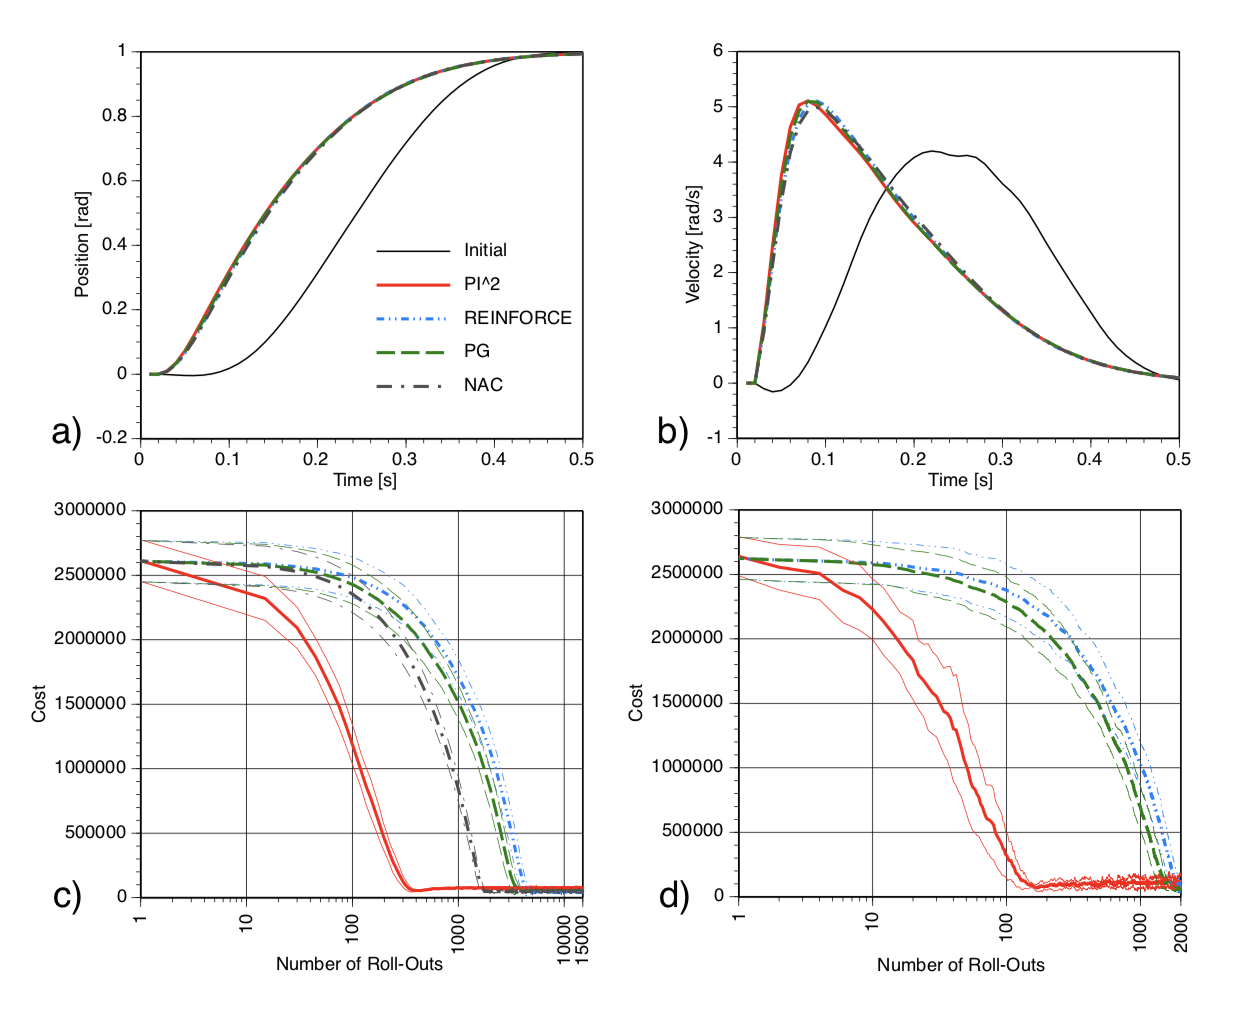
\includegraphics[width = .5\textwidth]{1dof}
  \caption{1 DOF comparison}
  \label{1dof}
\end{figure}


\subsubsection{Learning Optimal Performance of a 1 DOF Via-Point Task}
\ \\
Mostly the same but the cost function now forced the movement to pass through an intermediate via-point at $t = 300ms$. This is an abstract approximation of hitting a
target. The motor primitives were initialized to approximate a 5-th order polynomial as point-to-point movement,  called a minimum-jerk trajectory in the motor control literature.
The cost function was:

\begin{equation} 
  \begin{aligned}
    r_{300ms} &= 100000000(G- y_{t_{300ms}})^2 \\
    \phi_{t_N} &= 0  \nonumber 
  \end{aligned}
\end{equation}

with $G = 0.25$. Note that for this algorithm the PoWER algorithm can be applied too with a proper design of cost function.

The results are shown in $\ref{1dofv}$:

\begin{figure}[htbp]
  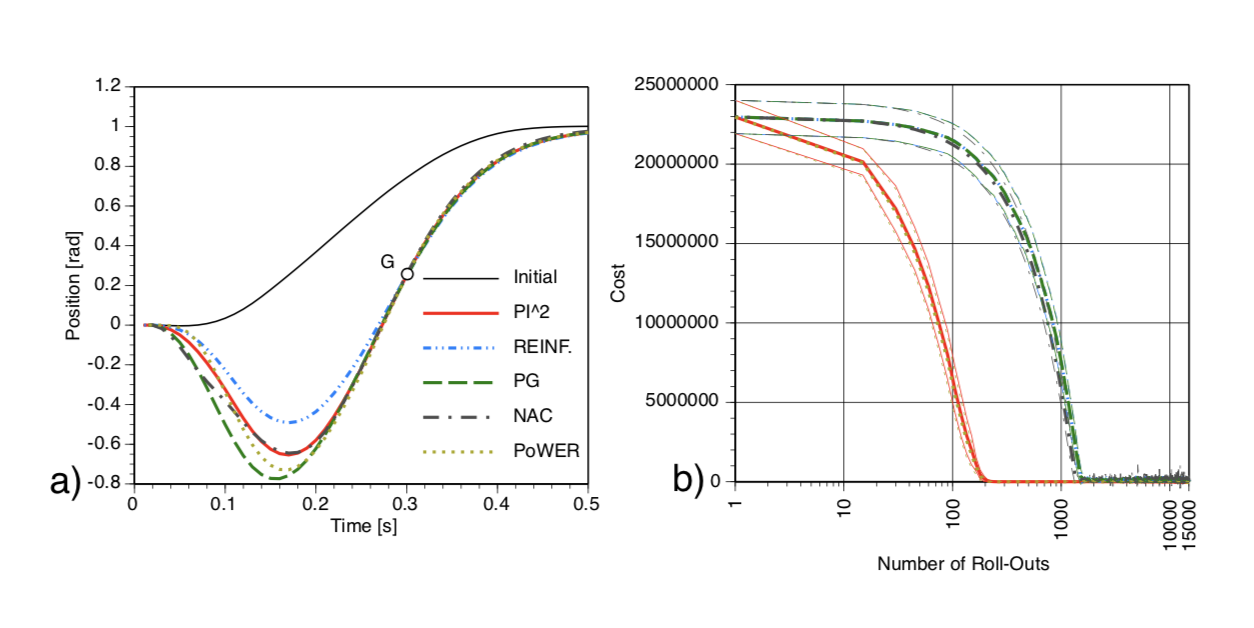
\includegraphics[width = .5\textwidth]{1dofv}
  \caption{1 DOF via-point comparison}
  \label{1dofv}
\end{figure}


\subsubsection{Learning Optimal Performance of a Multi-DOF Via-Point Task}
\ \\
Again the learning task was to pass through an intermediate target, just that a d = 2, 10, 50 dimensional motor primitive was employed thus result in a redundant learning 
problem. The implementation is done by assuming that the multi DOF system model plannar robot arms, where d links of equal length $l = 1/d$ are connected in an open chain
with recolute joints. Essentially the movement looks like a multi-segment snake in a plane whose tail is fixed at the origin, and the head of the snake can be moved in the 
2D plane by changing the joint angles between all the links.

To formalize this task as a reinforcement learning problem, we denote the joint angles of the robots as $\xi_i,\ i=1,\ldots,d $, s.t. the directly actuated part is: 
$\ddot{\xi_{i,t}} = f_{i, t} + g_{i, t}^{\top}(\theta_i + \epsilon_{i,t})$, The end-effector position is computed as: 

\begin{equation}
  \begin{aligned}
    x_t = \frac{1}{d} \sum_{i=1}^{d}\cos(\sum_{j=1}^{i}\xi_{j,t}) \\
    y_t = \frac{1}{d} \sum_{i=1}^{d}\sin(\sum_{j=1}^{i}\xi_{j,t}) \nonumber 
  \end{aligned}
\end{equation}


The cost function was designed as:


\begin{equation} 
  \begin{aligned}
    r_t &= \frac{\sum_{i=1}^{d}(d+1-i)(0.1f_{i,t}^2+ 0.5\theta_i^{\top}\theta_i)}{\sum_{i=1}^{d}(d+1-i)} \\
    \Delta r_{300ms} &= 10^8((0.5 - x_{t_{300ms}})^2+(0.5 - y_{t_{300ms}})^{2})  \nonumber \\ 
    \phi_{t_N} &= 0 
  \end{aligned}
\end{equation}

The comparison results shown in $\ref{mdofv}$

\begin{figure}[htbp]
  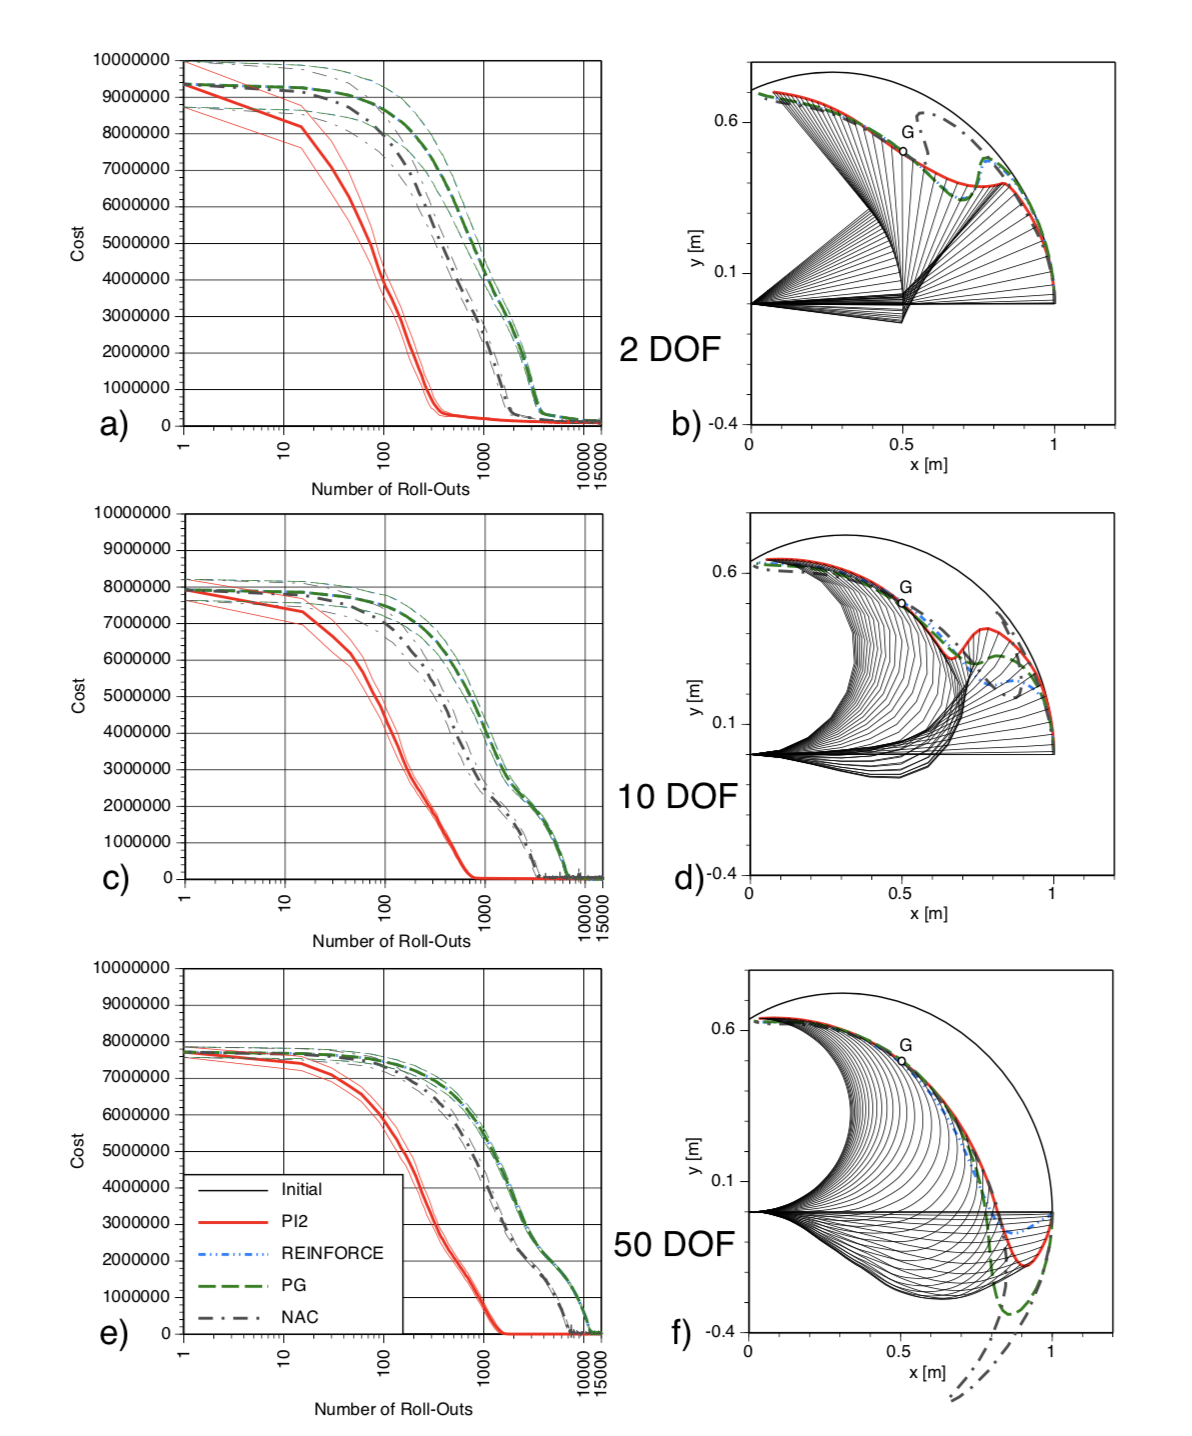
\includegraphics[width = .5\textwidth]{mdofv}
  \caption{multi-DOF via-point comparison}
  \label{mdofv}
\end{figure}

\subsubsection{Dog jumping}
\ \\
The robot dog is to jump across as gap. The paper only uses a simulation to show the results as real robot was not available. 
The dog has 3 DOFs per leg, thus a total of d=12, each DOF represented with 50 basis functions. 

PI$^2$ learning used primarily the forward progress as a reward, and slightly penalized the squared acceleration of each DOF, 
and the length of the parameter vector. Additionally, a penalty was incurred if the yaw or the roll exceeded a threshold value, which encouraged the
robot to jump straight across the gap instead of to the side or falling over. The exact cost design is:


\begin{equation} 
  \begin{aligned}
    r_t &= r_{roll}+ r_{yaw} + \sum_{i=1}^{d}(a_1 f_{i,t}^2 + 0.5a_2 \theta_i^{\top}\theta_i) \\
  r_{roll} &= \left\{ \begin{array}{rcl} &100(|roll_t|-0.3)^2 & if |roll_t|>3 \\ &0 &otherwise \end{array} \right. \nonumber \\ 
  r_{yaw} &= \left\{ \begin{array}{rcl} &100(|yaw_t|-0.1)^2 & if |yaw_t|>0.1 \\ &0 &otherwise \end{array} \right. \nonumber \\
    \phi_{t_N}& = 5 \times 10^{4} (goal -x_{nose})^2,   
  \end{aligned}
\end{equation}


Roll and yaw are the roll and yaw angles of the robot's body, and $x_{nose}$ is the position of the "nose".
The multipliers for each reward component were tuned to have a balanced influence of all terms. Ten learning trials were performed initially for the first parameter update.
 The best 5 trials were kept, and five additional new trials were performed for the second and all subsequent updates. 
Essentially, this method performs importance sampling, as the rewards for the 5 trials in memory were re-computed with the latest parameter vectors. 
A total of 100 trials was performed per run, and ten runs were collected for computing mean and standard deviations of learning curves.

\begin{figure}[htbp]
  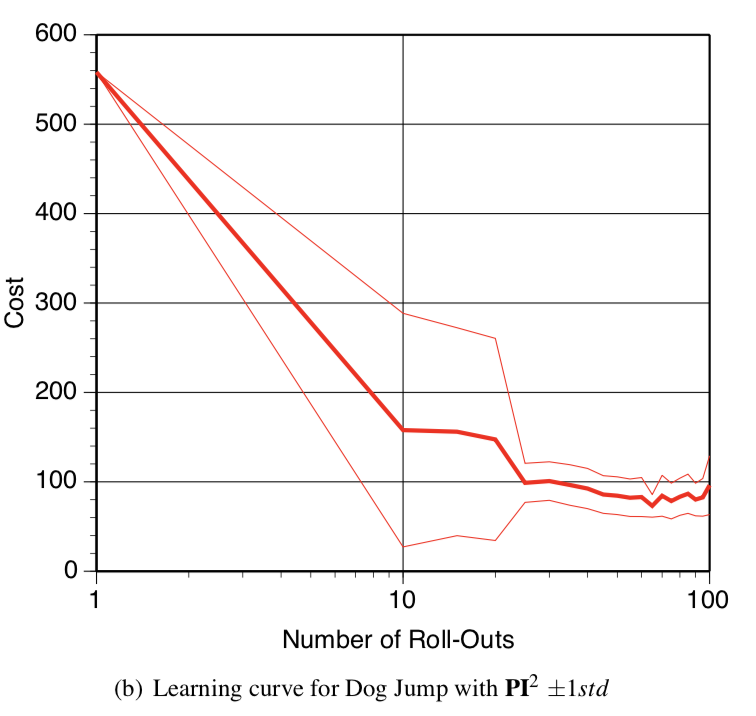
\includegraphics[width = .5\textwidth]{dog}
  \caption{learning curve}
  \label{dog}
\end{figure}

It should be noted that manual tuning is focused on generating a good cost function, which is beyond the scope of reinforcement learning. 


\section{Conclusion}
\ \\
Sevreral discussions are presented at the end of the paper.

\subsection{The Simplification $\lambda R^{-1} = \Sigma_{\epsilon}$}

In order to obtain linear 2nd order differential equations for the exponentially transformed HJB equations, the simplification $\lambda R^{-1} = \Sigma_{\epsilon}$ was applied.
Algorithmically, this assumption transforms the Gaussian probability for state transitions into a quadratic command cost, which is exactly what the immediate reward function postulated.
The future work is to remove the assummption by applying generalized Feynman-Kac Lemma.


\subsection{Model-based, Hybrid, and Model-free Learning}

The roll-outs, needed for computing the optimal controls, can be generated either from simulating a model, or by gathering experience from an actual system. In the latter case, 
only the control transition matrix of the model needs be known, such that we obtain a hybrid model-based/model-free method. The paper even went further and interpreted 
the stochastic dynamic system as a parameterized control policy, such that no knowledge of the model of the control system was needed anymore—that is, we entered a model-free learning domain



\subsection{Rules of Cost Function Design}


The cost functions allowed in our formulations can have arbitrary state cost, but need quadratic command cost. This is somewhat restrictive, although the user can be flexible in what is defined as a command.

The authors also numerically experimented with violations of the clean distinction between state and
command cost. The cost function can actually be replaced by an arbitary function of the state and command cost, and PI$^2$ somehow worked just fine in this improper setting.


What is more, it appears that the path integral formalism and the PI2 algorithm allow the user to exploit creativity in designing cost functions, without absolute need to adhere perfectly to the theoretical framework.


\subsection{Dealing with Hidden State}

There are 2 kinds of hidden states, deterministic ones that do not contributes to the probability roll-outs and stochastic ones that contributes to the passive dynamics. regarding the first category the paper already showed how it can be dropped out of the equation 
as they are termed as "non-directly actuated" parts. The second category is unobservable, yet it contributes to the system dynamics as a noise. Due to these stochastic differentiated hidden states, the results derived 
from PI$^2$ might be sub-optimal instead.


\subsection{Arbitrary States in the Cost Function}

It should be emphasized that the state cost $q_t$ can be any deterministic function of the state, that is, anything that is predictable from knowing the state, even if we do not know the predictive function. 
There is a lot of flexibility in this formulation, but it is also more restrictive than other approaches,
 for example, like policy gradients or the PoWER algorithm, where arbitrary variables can be used in the cost, no matter whether they are states or not.

 We can think of any variable that we would like to use in the cost as having a corresponding differential equation in the system dynamics, that is, we simply add these variables as state variables, just that we do not know the analytical form of these equations. 
 As in the previous section, it is useful to distinguish whether these states have deterministic or stochastic differential equations.

\subsection{*Discussion}

Here are some discussions about the previous lemma.

\subsubsection{Feynman-Kac lemma}

Copied from wiki:" The Feynman–Kac formula named after Richard Feynman and Mark Kac, establishes a link between parabolic partial differential equations (PDEs) and stochastic processes. 
When Mark Kac and Richard Feynman were both Cornell faculty, Kac attended a lecture of Feynman's and remarked that the two of them were working on the same thing from different directions. 
The Feynman-Kac formula resulted, which proves rigorously the real case of Feynman's path integrals. The complex case, which occurs when a particle's spin is included, is still unproven."


The theorem of ito's diffusion goes as follows:

Consider a PDE of this form:

\begin{equation}
\frac{\partial u(x, t)}{\partial t} + \sum_{i=1}^{N}\mu(x,t) \frac{\partial u}{\partial x}(x, t) + \frac{1}{2}\sum_{i=0}^{N} \sum_{j=0}^{N}\gamma_{i,j}(x,t) \frac{\partial^2 u}{\partial x_{i} \partial x_{j}}(x,t) - r(x,t)u(x,t)+f(x,t) = 0 \nonumber
\end{equation}

Where $\gamma_{x,t} = \sum_{k=1}^{N}\sigma_{i,k}(x,t)\sigma_{jk}(x,t)$, i.e. $\gamma = \sigma \sigma^{\top}$, $u: R^{N} \times [0,T] \to R$.  

The solution can be written as a conditional expectation:

\begin{equation}
  E^{Q} [\int_{t}^{T}e^{-\int_{t}^{T}V(X_{\tau}, \tau)d\tau}f(X_{\tau},r)dr+ e^{-\int_{t}^{T}V(X_{\tau}, \tau)d\tau} \Psi(X_{T})|X_t = x] \nonumber
\end{equation}

In our case we don't have $f(X_{\tau},\tau)$ term. Note that this expectation formula can be approximated using Monte Carlo or quasi-Monte Carlo methods, which is the method for numerical integration using discrepancy sequence instead of pseudorandom sequences.


\subsubsection{Eular scheme and Ito's lemma}

Because a Gaussian white noise $\xi$ or $\xi(\psi)$ is a generalized stochastic process such that there exists a Wiener process $W(t) t\in T$ satisfying $\xi(t) = \frac{dW(t)}{dt}$, according to Ito's
lemma, when we are doing second order Taylor approximation around the point of some stage, the term $dW^2(t) = dt$, that's essentially why we follow the Eular scheme to simulate a stochastic process. (Here we ignored some computational details) 


\subsubsection{Fisher information matrix}

The fisher information is a way of measuring the amount of information that an observable random variable X carries about an unknown parameter $\theta$ upon which the probability of X depends.
When there are N parameters, $\theta \in R^{N \times 1}$, the fisher information matrix takes form of N by N matrix,
with element:

\begin{equation}
  [I(\theta)]_{i,j} = E[(\frac{\partial}{\partial \theta_i} \log f(X ; \theta))(\frac{\partial}{\partial \theta_j} \log f(X ; \theta))| \theta] \nonumber
\end{equation}

FIM is a N by N positive semi-definite matrix.


\subsection{Final conclusion}

As can be seen from the previous figures, the PI$^2$ Algorithm has a surprisingly good performance, without any need for tuning parameters. And it's scalable to high dimensionality.
Yet there's indeed space to improve such as the cost function design, which future work might be focus on to move the algorithm to a "black box" character.

% if have a single appendix:
%\appendix[Proof of the Zonklar Equations]
% or
%\appendix  % for no appendix headi
% do not use \section anymore after \appendix, only \section*
% is possibly needed

% use appendices with more than one appendix
% then use \section to start each appendix
% you must declare a \section before using any
% \subsection or using \label (\appendices by itself
% starts a section numbered zero.)
%




% you can choose not to have a title for an appendix
% if you want by leaving the argument blank



% use section* for acknowledgment



% Can use something like this to put references on a page
% by themselves when using endfloat and the captionsoff option.
\ifCLASSOPTIONcaptionsoff
  \newpage
\fi



% trigger a \newpage just before the given reference
% number - used to balance the columns on the last page
% adjust value as needed - may need to be readjusted if
% the document is modified later
%\IEEEtriggeratref{8}
% The "triggered" command can be changed if desired:
%\IEEEtriggercmd{\enlargethispage{-5in}}

% references section

% can use a bibliography generated by BibTeX as a .bbl file
% BibTeX documentation can be easily obtained at:
% http://mirror.ctan.org/biblio/bibtex/contrib/doc/
% The IEEEtran BibTeX style support page is at:
% http://www.michaelshell.org/tex/ieeetran/bibtex/
%\bibliographystyle{IEEEtran}
% argument is your BibTeX string definitions and bibliography database(s)
%\bibliography{IEEEabrv,../bib/paper}
%
% <OR> manually copy in the resultant .bbl file
% set second argument of \begin to the number of references
% (used to reserve space for the reference number labels box)
\begin{thebibliography}{1}

\bibitem{Theodo}Theodorou, Evangelos, Jonas Buchli, and Stefan Schaal. "A generalized path integral control approach to reinforcement learning." journal of machine learning research 11.Nov (2010): 3137-3181.

\end{thebibliography}





\end{document}


